\documentclass[10pt,ignorenonframetext,]{beamer}
\setbeamertemplate{caption}[numbered]
\setbeamertemplate{caption label separator}{: }
\setbeamercolor{caption name}{fg=normal text.fg}
\beamertemplatenavigationsymbolsempty
\usepackage{lmodern}
\usepackage{amssymb,amsmath}
\usepackage{ifxetex,ifluatex}
\usepackage{fixltx2e} % provides \textsubscript
\ifnum 0\ifxetex 1\fi\ifluatex 1\fi=0 % if pdftex
  \usepackage[T1]{fontenc}
  \usepackage[utf8]{inputenc}
\else % if luatex or xelatex
  \ifxetex
    \usepackage{mathspec}
  \else
    \usepackage{fontspec}
  \fi
  \defaultfontfeatures{Ligatures=TeX,Scale=MatchLowercase}
\fi
\usetheme[]{CambridgeUS}
\usecolortheme{dove}
\usefonttheme{structurebold}
% use upquote if available, for straight quotes in verbatim environments
\IfFileExists{upquote.sty}{\usepackage{upquote}}{}
% use microtype if available
\IfFileExists{microtype.sty}{%
\usepackage{microtype}
\UseMicrotypeSet[protrusion]{basicmath} % disable protrusion for tt fonts
}{}
\newif\ifbibliography
\hypersetup{
            pdftitle={Predicting crime rates using taxi rides in NYC},
            pdfborder={0 0 0},
            breaklinks=true}
\urlstyle{same}  % don't use monospace font for urls

% Prevent slide breaks in the middle of a paragraph:
\widowpenalties 1 10000
\raggedbottom

\AtBeginPart{
  \let\insertpartnumber\relax
  \let\partname\relax
  \frame{\partpage}
}
\AtBeginSection{
  \ifbibliography
  \else
    \let\insertsectionnumber\relax
    \let\sectionname\relax
    \frame{\sectionpage}
  \fi
}
\AtBeginSubsection{
  \let\insertsubsectionnumber\relax
  \let\subsectionname\relax
  \frame{\subsectionpage}
}

\setlength{\parindent}{0pt}
\setlength{\parskip}{6pt plus 2pt minus 1pt}
\setlength{\emergencystretch}{3em}  % prevent overfull lines
\providecommand{\tightlist}{%
  \setlength{\itemsep}{0pt}\setlength{\parskip}{0pt}}
\setcounter{secnumdepth}{0}
\author{Carlos Petricioli \and
    Varsha Muralidharan   \and
    Valerie Angulo  }

\institute[New York University]{ New York University \\ \{cpa253,vm1370,vaa238\}@nyu.edu }

\setbeamerfont{headline}{size=\fontsize{8}{1}\selectfont}
\setbeamertemplate{headline}
{
  \leavevmode%
  \hbox{%
  \begin{beamercolorbox}[wd=1\paperwidth,ht=2.3ex,dp=1.5ex,right]{section in head/foot}%
    \usebeamerfont{section in head/foot}\insertsectionhead\hspace*{1ex}
  \end{beamercolorbox}%
  % \begin{beamercolorbox}[wd=0\paperwidth,ht=2.65ex,dp=1.5ex,right]{subsection in head/foot}%
  %   \usebeamerfont{subsection in head/foot}\hspace*{2ex}\insertsubsectionhead
  % \end{beamercolorbox}
  }%
  \vskip0pt%
}


% \setbeamertemplate{navigation symbols}{}
% \setbeamertemplate{footline}[page number]
\setbeamertemplate{footline}
{
  \leavevmode%
  \hbox{%
      \begin{beamercolorbox}[wd=1\paperwidth,ht=2.25ex,dp=1ex,right]{author in head/foot}%
          \usebeamerfont{author in head/foot}
          \insertframenumber{} of  \inserttotalframenumber\hspace*{2ex} 
      \end{beamercolorbox}}%
      \vskip0pt%
}

% Set Color ==============================
% Custom colors
\usepackage{xcolor}

%\definecolor{gold}{HTML}{FDD017}
\definecolor{gold}{HTML}{fdde5c}
% \definecolor{deep sky blue}{HTML}{3BB9FF}
% \definecolor{light sky blue}{HTML}{82CAFA}

\makeatletter
\definecolor{mybackground}{HTML}{fef5d0}
\definecolor{myforeground}{HTML}{0000A0}

\setbeamercolor{normal text}{fg=black,bg=white}
\setbeamercolor{alerted text}{fg=red}
\setbeamercolor{example text}{fg=black}

\setbeamercolor{block title}{bg=mybackground,fg=black}


\setbeamercolor{background canvas}{fg=myforeground, bg=white}
\setbeamercolor{background}{fg=myforeground, bg=mybackground}

\setbeamercolor{palette primary}{fg=black, bg=gray!30!white}
\setbeamercolor{palette secondary}{fg=black, bg=gray!20!white}
\setbeamercolor{palette tertiary}{fg=black, bg=gold}
\makeatother

\title{Predicting crime rates using taxi rides in NYC}
\date{12/15/2017}

\begin{document}
\frame{\titlepage}

\begin{frame}{Big Data Analytics Symposium - Fall 2017}

\begin{block}{Analytics Project}

Predicting crime rates using taxi rides in NYC

\end{block}

\begin{block}{Team}

\begin{itemize}
\item
  Carlos Petricioli (cpa253)
\item
  Varsha Muralidharan (vm1370)
\item
  Valerie Angulo (vaa238)
\end{itemize}

\end{block}

\begin{block}{Abstract}

\begin{itemize}
\tightlist
\item
  Our study looks at the relationship between crime rates and taxi usage
  in New York City.
\item
  Our hypothesis is that people are less likely to walk in areas
  subjectively deemed more dangerous and will instead opt to use more
  reliable and immediate transportation such as designated taxis.
\item
  WE FOUND THAT \_\_\_\_.
\end{itemize}

\end{block}

\end{frame}

\begin{frame}{Motivation}

\begin{block}{Typical users of this application}

The scientific community, law enforcement, those in public
transportation

\end{block}

\begin{block}{Beneficiaries of this application}

Members of the community and tourists, law enforcement

\end{block}

\begin{block}{Importance of this analytic}

\begin{itemize}
\tightlist
\item
  This analytic can help law enforcement predict areas of crime based on
  New Yorkers transportation habits. Law enforcement officials may be
  able to predict which areas will have a higher rate of crime in the
  future.
\item
  People who live in an area are aware of the safety of their
  surroundings and this awareness can be represented by how comfortable
  residents may be in walking or taking the subway versus taking more
  immediate, more expensive, modes of transportation such as taxis.
\item
  This analytic can benefit the community and tourists by influencing
  their current and future transportation behaviors
\end{itemize}

\end{block}

\end{frame}

\begin{frame}{Goodness}

What steps were taken to assess the `goodness' of the analytic?\\
\textless{} Short description of why you believe the results of your
analytic are correct and can be trusted

\begin{block}{cleaning data}

\begin{itemize}
\tightlist
\item
  we made sure that taxi columns with indeterminable dates were not
  included and that the columns for all years matched.
\item
  we made sure taxi, crime and weather data could be related by zone
\end{itemize}

\end{block}

\begin{block}{model testing}

we made sure that --

\end{block}

\end{frame}

\begin{frame}{Data Sources}

\begin{block}{Taxi rides data form TLC
\href{http://www.nyc.gov/html/tlc/html/about/trip_record_data.shtml}{(\emph{Link})}}

\begin{itemize}
\item
  It covers years from 2009 to June 2017.
\item
  Data Size: 230 GB .. 2 TB
\item
  The yellow taxi trip records include:
\item
  pick-up and drop-off dates/times,
\item
  pick-up and drop-off locations,
\item
  trip distance,
\item
  itemized fares,
\item
  rate types,
\item
  payment type,
\item
  passenger counts.
\end{itemize}

\end{block}

\end{frame}

\begin{frame}

\begin{block}{NYPD Complaint Data
\href{https://data.cityofnewyork.us/Public-Safety/NYPD-Complaint-Data-Historic/qgea-i56i}{(\emph{Link
1,}}
\href{https://data.cityofnewyork.us/Public-Safety/NYPD-Complaint-Data-Current-YTD/5uac-w243}{\emph{Link
2)}}}

\begin{itemize}
\tightlist
\item
  This dataset includes all valid felony, misdemeanor, and violation
  crimes reported to the New York City Police Department (NYPD) from
  2006 to year to date data.
\end{itemize}

-Data Size: 1.5 GB

\end{block}

\begin{block}{NOAA Weather stations data
\href{https://www.ncdc.noaa.gov/isd}{\emph{(Link)}}}

The \emph{Integrated Surface Database (ISD)} consists of global hourly
ansynoptic observations compiled from numerous sources into a single
common ASCII format and common data model.

\begin{itemize}
\item
  ISD's complete history of hour-by-hour readings for one user-specified
  weather stations
\item
  We selected:
\item
  Central Park
\item
  JFK
\item
  Laguardia
\end{itemize}

-Data Size: 165 MB

\end{block}

\end{frame}

\begin{frame}{Design Diagram}

\begin{center}
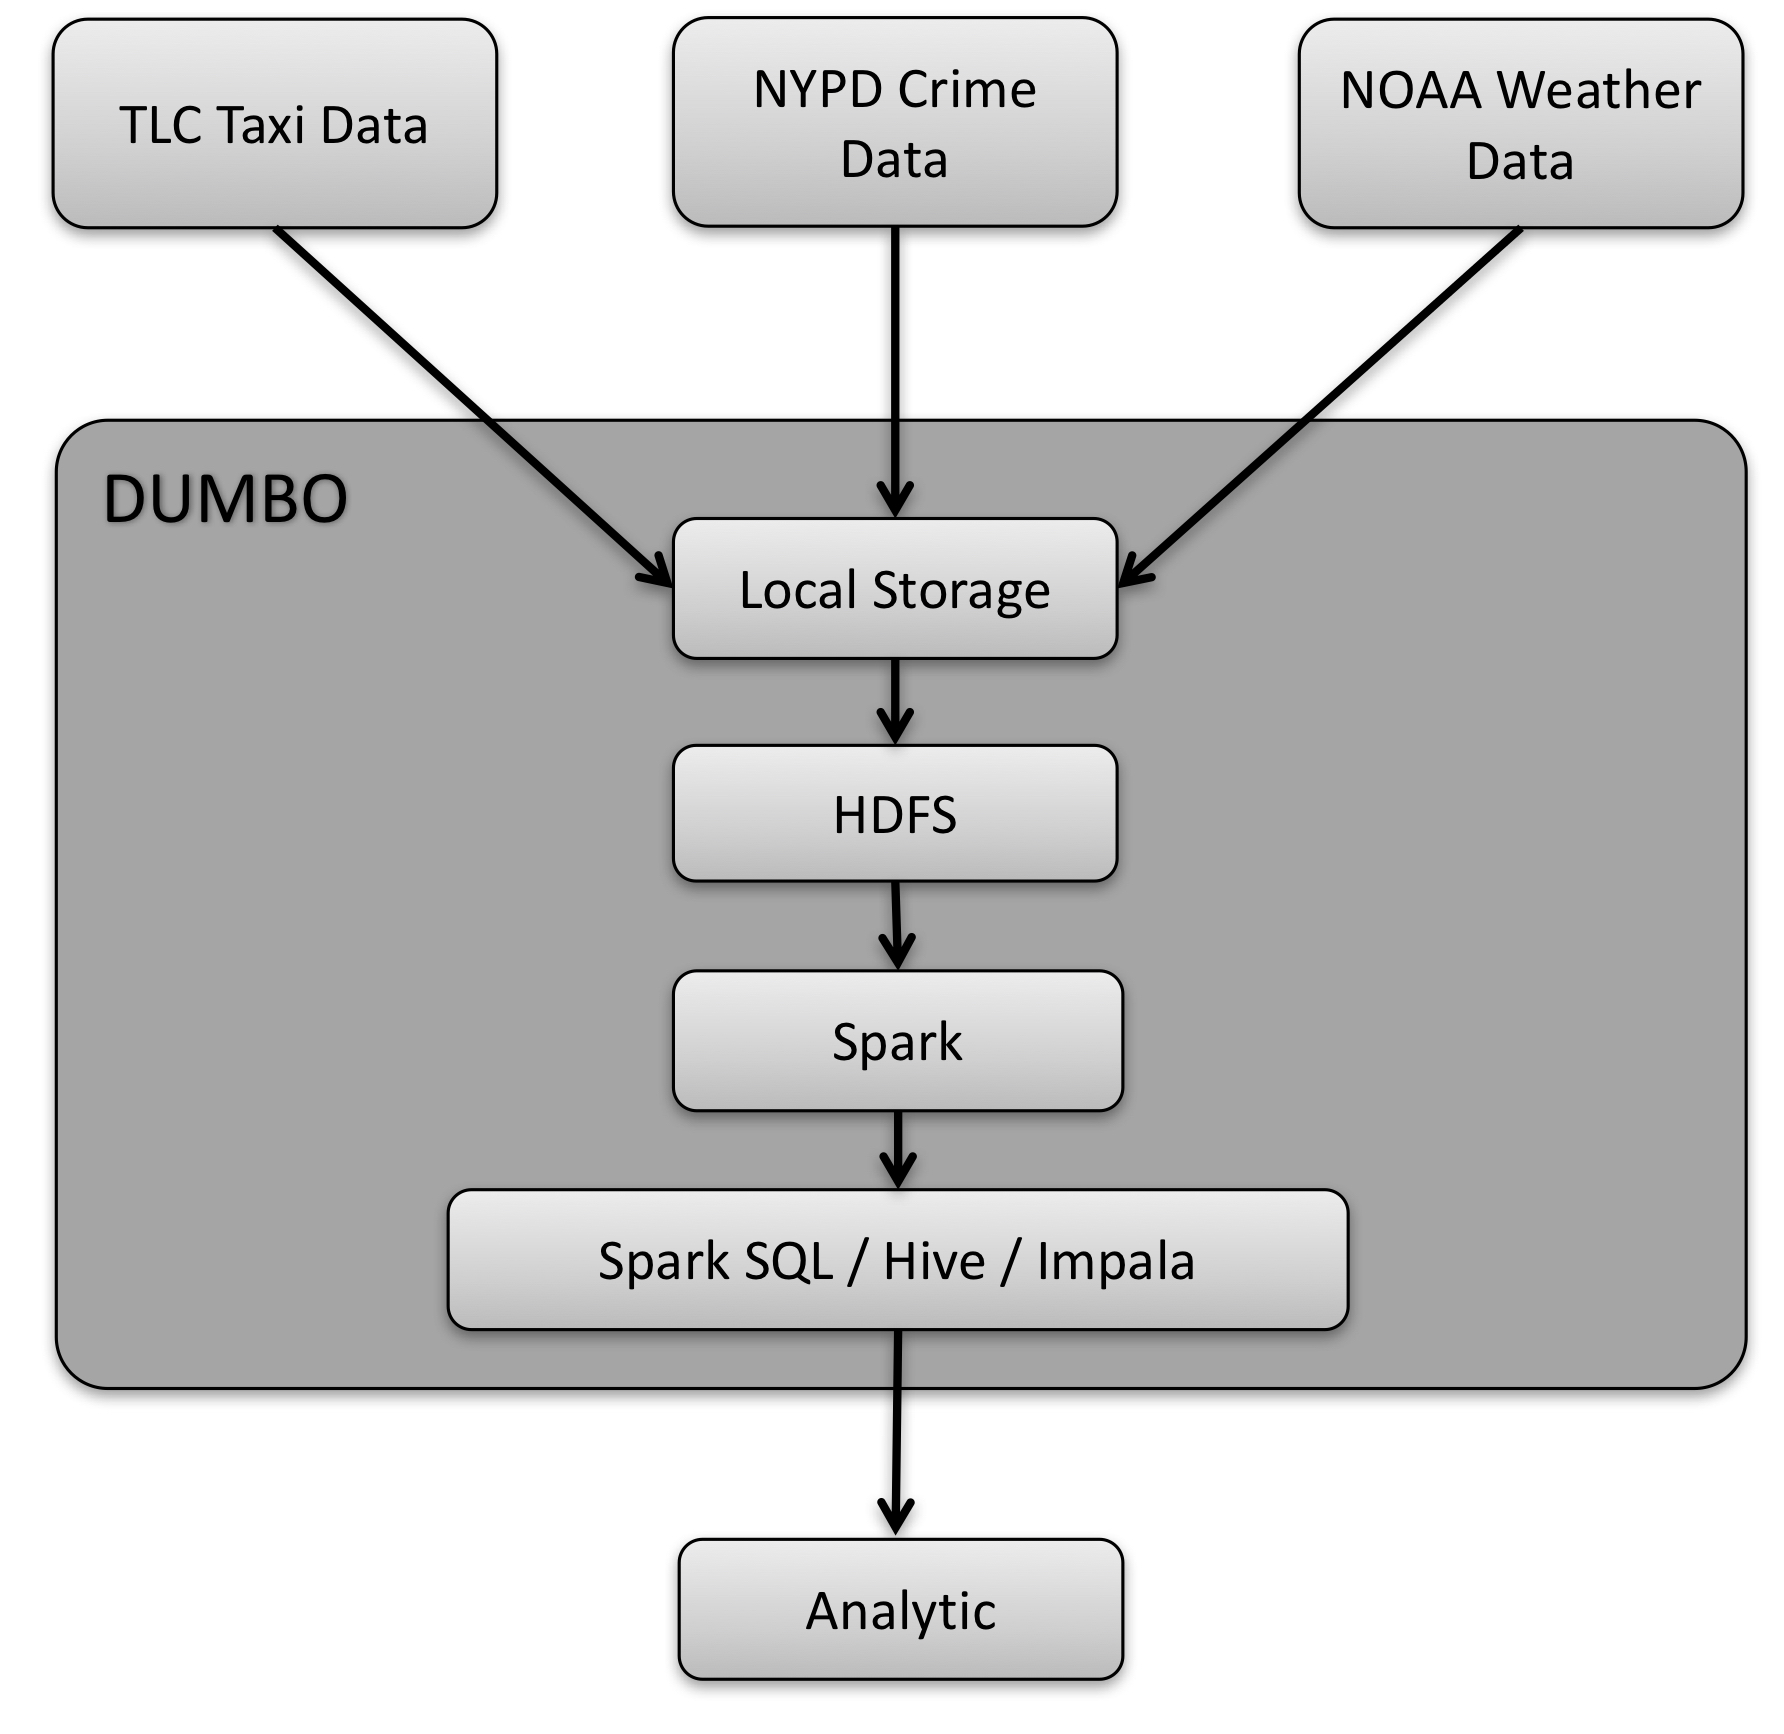
\includegraphics[height=.6\textheight]{img/DesignFlowDiagram.jpg}
\end{center}

\begin{block}{Platform:}

\begin{itemize}
\tightlist
\item
  NYU HPC cluster (Dumbo)
\end{itemize}

\end{block}

\end{frame}

\begin{frame}{Results}

3 results, insights, observations, outcomes

\begin{enumerate}
\def\labelenumi{\arabic{enumi}.}
\item
  Result 1
\item
  Result 2
\item
  Result 3
\end{enumerate}

\end{frame}

\begin{frame}{Obstacles}

\begin{enumerate}
\def\labelenumi{\arabic{enumi}.}
\item
  Cleaning the data- The taxi data was the most challenging to clean due
  to its size and inconsistencies in columns for specific years. Some
  years were unable to be determined and were excluded for the taxi data
  set.
\item
  Joining the data- Designated taxi zones were determined for taxi
  pickup locations and crime locations in order to join the crime and
  taxi data sets and an hourly\_date column was added to join taxi and
  weather data sets
\end{enumerate}

\end{frame}

\begin{frame}{Summary}

\begin{itemize}
\tightlist
\item
  We collected NYC taxi trip data, NYC crime data and weather data from
  Central Park, JFK and LaGuardia
\item
  We joined together the data sets through taxi zones (taxi\_zone\_id)
  and hourly\_data
\item
  Our main questions revolve around whether taxi usage depends on crime
  rate in a specific zone, how much weather plays a part in the
  relationship between taxi usage and crime and how the distance of the
  trip affects taxi usage in relationship to crime
\item
  WE FOUND THAT \_\_\_\_\_\_\_\_\_\_\_\_\_\_
\end{itemize}

Brief wrap-up!

\end{frame}

\begin{frame}{Acknowledgements}

Thank you to everyone at NYU HPC Support for helping us with questions
and problems we encountered during this project. Special thanks to
Santhosh Konda \href{mailto:hpc@nyu.edu}{\nolinkurl{hpc@nyu.edu}} for
responding so quickly to our e-mails!

\end{frame}

\begin{frame}{References}

\begin{thebibliography}{1}

\bibitem{Bendler14}
J.~Bendler, T.~Brandt, S.~Wagner, and D.~Neumann.
\newblock Investigating crime-to-twitter relationships in urban environments -
  facilitating a virtual neighborhood watch.
\newblock In M.~Avital, J.~M. Leimeister, and U.~Schultze, editors, {\em ECIS},
  2014.

\bibitem{Wang16}
H.~Wang, D.~Kifer, C.~Graif, and Z.~Li.
\newblock Crime rate inference with big data.
\newblock In {\em Proceedings of the 22Nd ACM SIGKDD International Conference
  on Knowledge Discovery and Data Mining}, KDD '16, pages 635--644, New York,
  NY, USA, 2016. ACM.

\bibitem{Traunmueller14}
M.~Traunmueller, G.~Quattrone, and L.~Capra.
\newblock {\em Mining Mobile Phone Data to Investigate Urban Crime Theories at
  Scale}, pages 396--411.
\newblock Springer International Publishing, Cham, 2014.
\end{thebibliography}

\end{frame}

\begin{frame}

\begin{thebibliography}{1}
\bibitem{OUAC}
A.~Bogomolov, B.~Lepri, J.~Staiano, N.~Oliver, F.~Pianesi, and A.~Pentland.
\newblock Once upon a crime: Towards crime prediction from demographics and
  mobile data, Sep 2014.

\bibitem{Chainey}
S.~Chainey, L.~Tompson, and S.~Uhlig.
\newblock {The Utility of Hotspot Mapping for Predicting Spatial Patterns of
  Crime}.
\newblock {\em Security Journal}, 21(1-2):4--28, Feb 2008.

\bibitem{visCrime}
T.~Nakaya and K.~Yano.
\newblock Visualising crime clusters in a space-time cube: An exploratory
  data-analysis approach using space-time kernel density estimation and scan
  statistics.
\newblock {\em Transactions in GIS}, 14(3):223--239, 2010.
\end{thebibliography}

\end{frame}

\section{Thank you!}\label{thank-you}

\end{document}
